\documentclass[12pt,a4paper,titlepage,final]{article}

% cestina a fonty
\usepackage[czech]{babel}
\usepackage[utf8]{inputenc}
% balicky pro odkazy
\usepackage[bookmarksopen,colorlinks,plainpages=false,urlcolor=blue,unicode]{hyperref}
\usepackage{url}
% obrazky
\usepackage[dvipdf]{graphicx}
\usepackage{rotating}
% velikost stranky
\usepackage[top=3.5cm, left=2.0cm, text={17cm, 24cm}, ignorefoot]{geometry}
%více řádkové tabulky
\usepackage{multirow}
\usepackage{tabularx}
\usepackage{colortbl}
%barvy
\usepackage[table]{xcolor}
%ostatní
\usepackage{textcomp}
\usepackage{tipa}
\usepackage{float}

%vlastni prikazy
\newcommand{\myuv}[1]{\quotedblbase #1\textquotedblleft}
\newcommand{\jEQ}{\scriptsize{===}}
\newcommand{\nEQ}{\scriptsize{!==}}
\newcommand{\ME}{$<$\cellcolor{blue!10}}
\newcommand{\VE}{$>$\cellcolor{yellow!15}}
\newcommand{\RO}{$=$\cellcolor{green!15}}
\newcommand{\PR}{\cellcolor{red!15}}
\newcommand{\exitem}[1]{\textlangle \emph{#1}\textrangle}
\newcommand{\sipka}{$\rightarrow$}
\newcommand{\slozav}[1]{\textbf{\textbraceleft}#1\textbf{\textbraceright}}
\newcommand{\kulzav}[1]{\textbf{(}#1\textbf{)}}


\begin{document}

%%%%%%%%%%%%%%%%%%%%%%%%%%%%%%%%%%%%%%%%%%%%%%%%%%%%%%%%%%%%%%%%%%%%%%%%%%%%%%
% titulní strana

% !!!!!!!!!!!!!!!!!!!!!!!!!!!!!!!!!!!!!!!!!!!!!!!!!
\def\authorA{Horký Lukáš}
\def\loginA{xhorky21}
\def\authorB{Hurta Marek}
\def\loginB{xhurta01}
\def\authorC{Huták Lukáš}
\def\loginC{xhutak01}
\def\authorD{Kozubík Michal}
\def\loginD{xkozub03}
\def\authorE{Lietavcová Zuzana}
\def\loginE{xlieta00}
\def\projname{Implementace interpretu imperativního jazyka IFJ13}
% !!!!!!!!!!!!!!!!!!!!!!!!!!!!!!!!!!!!!!!!!!!!!!!!!

\begin{titlepage}

% \vspace*{1cm}
\begin{figure}[!h]
  \centering
  \includegraphics[height=5cm]{img/logo.eps}
\end{figure}

\vfill

\begin{center}
\begin{Large}
Dokumentace k projektu pro předměty IFJ a IAL\\
\end{Large}
\bigskip
\begin{Huge}
\projname\\
\end{Huge}
\begin{large}
Tým \texttt{020}, varianta \texttt{a/2/II}
\end{large}
\end{center}

\vspace{4pt}

\begin{center}
\begin{large}
Implementovaná rozšíření \\
\texttt{MINUS}, \texttt{FUNEXP}, \texttt{ELSEIF}
\end{large}
\end{center}

\vfill

\begin{center}
\begin{Large}
\today
\end{Large}
\end{center}

\vfill

\begin{flushleft}
\begin{large}
\begin{tabular}{llll}
Autoři: & \authorA, & \qquad \texttt{\loginA} & \qquad 20\,\% \\
 & \authorB, & \qquad \texttt{\loginB} & \qquad 20\,\%\\
 & \authorC \ (vedoucí týmu), & \qquad \texttt{\loginC} & \qquad 20\,\%\\
 & \authorD, & \qquad \texttt{\loginD} & \qquad 20\,\% \\
 & \authorE & \qquad \texttt{\loginE} & \qquad 20\,\%\\
 & Fakulta Informačních Technologií & \\
 & Vysoké Učení Technické v~Brně
\end{tabular}
\end{large}
\end{flushleft}
\end{titlepage}


%%%%%%%%%%%%%%%%%%%%%%%%%%%%%%%%%%%%%%%%%%%%%%%%%%%%%%%%%%%%%%%%%%%%%%%%%%%%%%
% obsah
\pagestyle{plain}
\pagenumbering{roman}
\setcounter{page}{1}
\tableofcontents

%%%%%%%%%%%%%%%%%%%%%%%%%%%%%%%%%%%%%%%%%%%%%%%%%%%%%%%%%%%%%%%%%%%%%%%%%%%%%%
% textova zprava
\newpage
\pagestyle{plain}
\pagenumbering{arabic}
\setcounter{page}{1}

%%%%%%%%%%%%%%%%%%%%%%%%%%%%%%%%%%%%%%%%%%%%%%%%%%%%%%%%%%%%%%%%%%%%%%%%%%%%%%
\section{Úvod} \label{uvod}
%%%%%%%%%%%%%%%%%%%%%%%%%%%%%%%%%%%%%%%%%%%%%%%%%%%%%%%%%%%%%%%%%%%%%%%%%%%%%%

Tento dokument popisuje implementaci interpretu jazyka IFJ13 a průběh jeho
vývoje. Jelikož se jedná o komplexní projekt vyžadující účast více členů, není
řešení zcela jednoduché a~naráží na nutnost pečlivého řízení projektu. 

Dokumentace se skládá z několika částí. Kapitola \ref{tym}. pojednává o podobě 
průběhu vývoje a~metodách použitých při práci v týmu. O zjednodušeném návrhu 
struktury se lze dočíst v~kapitole \ref{navrhstrukt}. a konkrétní popis 
implementace jednotlivých součástí se nachází v navazující 
kapitole (\ref{implementace}). Testování se věnuje kapitola \ref{testovani}. a 
stručné závěrečné shrnutí projektu popisuje \ref{shrnuti}. kapitola. 
V~přílohách se nachází nákres konečného automatu lexikálního analyzátoru, 
precedenční tabulka a LL gramatika.

%%%%%%%%%%%%%%%%%%%%%%%%%%%%%%%%%%%%%%%%%%%%%%%%%%%%%%%%%%%%%%%%%%%%%%%%%%%%%%
\section{Práce v týmu} \label{tym}
%%%%%%%%%%%%%%%%%%%%%%%%%%%%%%%%%%%%%%%%%%%%%%%%%%%%%%%%%%%%%%%%%%%%%%%%%%%%%%
\subsection{Příprava a plánování}
%%%%%%%%%%%%%%%%%%%%%%%%%%%%%%%%%%%%%%%%%%%%%%%%%%%%%%%%%%%%%%%%%%%%%%%%%%%%%%
Před samotným zahájením semestru byl sestavený tým, ve kterém se jednotliví 
členové již důvěrně znali, a tudíž se nám podařilo předejít nepříjemným 
překvapením. Projekt nebyl brán na lehkou váhu, a proto po uveřejnění zadání 
byl nastolen režim (téměř) pravidelných týdenních schůzí, kterých se 
účastnili všichni členové. Schůze převážně spočívaly v analýze pokroku od~minulého 
setkání, řešení aktuálních technických otázek, návrhu společného 
rozhraní jednotlivých částí, které se později spojovaly do větších celků a 
rozdělení úkolů po vzájemné dohodě. Tento způsob řízení se zpětným pohledem 
jeví jako uspokojivý, neboť vedl k průběžnému pokroku. Aby se dosáhlo určitého 
sjednocení z pohledu tvorby kódu, byl zaveden styl zápisu programu 
vycházející z Linux Kernel Coding Style\cite{coding_style}. Bohužel se ne vždy 
podařilo jeho úplné dodržení a~docházelo proto k drobným odchylkám. Jako způsob 
komentování kódu byl zvolen styl pro~Doxygen.

%%%%%%%%%%%%%%%%%%%%%%%%%%%%%%%%%%%%%%%%%%%%%%%%%%%%%%%%%%%%%%%%%%%%%%%%%%%%%%
\subsection{Správa kódu a komunikace mezi členy}
%%%%%%%%%%%%%%%%%%%%%%%%%%%%%%%%%%%%%%%%%%%%%%%%%%%%%%%%%%%%%%%%%%%%%%%%%%%%%%
Při práce v týmu je důležitou součástí přístup k aktuální verzi projektu, 
se kterým přichází všichni členové do styku. Byl tedy zvolen nástroj GIT s 
privátním repositářem, jenž byl provozován na serveru Bitbucket, čímž bylo 
dosaženo kvalitního sdílení zdrojových kódu a dalších materiálů mezi všemi 
členy týmu. V rané fázi bylo uvažováno i o využití softwaru pro řízení 
projektů, ale od toho návrhu se ustoupilo, neboť kvůli relativně malému 
počtu členů se jevil neefektivní. Jako vhodná náhrada se využila zřízená 
soukromá skupina na sociální síti, která pomohla zrychlené komunikaci a 
efektivnímu řešení dodatečných problémů. Pro další komunikaci se užívaly 
různé formy instant messagingu včetně video hovorů.


%%%%%%%%%%%%%%%%%%%%%%%%%%%%%%%%%%%%%%%%%%%%%%%%%%%%%%%%%%%%%%%%%%%%%%%%%%%%%%
\section{Návrh struktury projektu} \label{navrhstrukt}
%%%%%%%%%%%%%%%%%%%%%%%%%%%%%%%%%%%%%%%%%%%%%%%%%%%%%%%%%%%%%%%%%%%%%%%%%%%%%%
V průběhu společných setkání při navrhování jednotlivých částí bylo jasné, 
že jen dobře navržený projekt může dosáhnout úspěšného výsledku. Struktura 
byla vytvářena postupně, protože žádný člen týmu neměl předchozí zkušenosti 
s tvorbou interpretu. V důsledku pečlivého návrhu docházelo pouze k drobným 
průběžným změnám. Jednotlivým částem se věnovali členové dle rozdělení úkolů 
s různou mírou zastoupení svého autorství a vzniklá struktura měla 
následující pojetí:

\begin{itemize}
	\item Scanner (Horký Lukáš, Huták Lukáš)
	\item Parser (Kozubík Michal)
	\item Generátor instrukcí (Hurta Marek, Lietavcová Zuzana)
	\item Interpret (Horký Lukáš, Huták Lukáš)
	\item Vestavěné funkce (všichni členové)
	\item IAL funkce (Hurta Marek, Kozubík Michal, Lietavcová Zuzana)
\end{itemize}

\begin{figure}
\begin{center}
  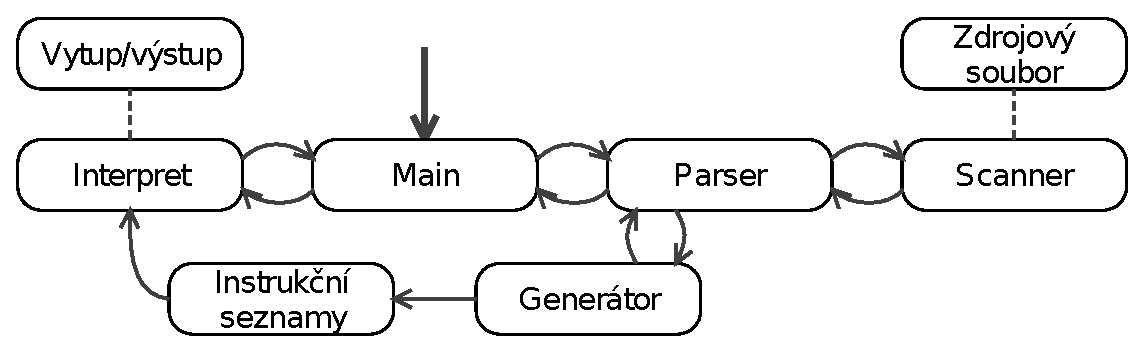
\includegraphics[scale = 0.7]{img/navrh.eps}
  \caption{Návrh struktury programu}
  \label{obr_navrh}
\end{center}
\end{figure}

Výsledná podoba je na obrázku \ref{obr_navrh}. Vzhledem k tomu, že vestavěné 
funkce jsou užívány zejména interpretem a IAL funkce interpretem a parserem, 
nejsou vyobrazeny samostatně, ale jsou vnímány jako vnitřní součásti 
jednotlivých celků.

%%%%%%%%%%%%%%%%%%%%%%%%%%%%%%%%%%%%%%%%%%%%%%%%%%%%%%%%%%%%%%%%%%%%%%%%%%%%%%
\section{Implementace} \label{implementace}
%%%%%%%%%%%%%%%%%%%%%%%%%%%%%%%%%%%%%%%%%%%%%%%%%%%%%%%%%%%%%%%%%%%%%%%%%%%%%%
Tato kapitola popisuje implementaci jednotlivých součásti, tak jak byly 
navrženy v předchozí kapitole. V každé části bylo dbáno na správné uvolňování 
paměti i v případě narušení činnosti vykonávání programu chybami způsobenými 
ve vstupním programu, apod.


%%%%%%%%%%%%%%%%%%%%%%%%%%%%%%%%%%%%%%%%%%%%%%%%%%%%%%%%%%%%%%%%%%%%%%%%%%%%%%
\subsection{Lexikální analyzátor (scanner)}
%%%%%%%%%%%%%%%%%%%%%%%%%%%%%%%%%%%%%%%%%%%%%%%%%%%%%%%%%%%%%%%%%%%%%%%%%%%%%%
Úkolem toho modulu je ze vstupní posloupnosti znaků vytvářet lexikální jednotky. 
Ty jsou reprezentovány ve formě tokenů, které jsou následně předány parseru k 
dalšímu zpracování. Lexikální analýza je realizována na základě konečného 
automatu (viz příloha \ref{scanner_graf}). Z hlediska implementace se užívá 
stavová proměnná a v následném přepínači switch se pak na základě načteného 
znaku a aktuálního stavu určí, do jakého stavu má lexikální analyzátor přejít 
a~případně zdali se nejedná o konečný stav.

Zároveň je potřeba občas načtené znaky ukládat do řetězcové struktury, protože
ve spoustě případů nestačí pro úspěšné vytvoření tokenu znát pouze konečný 
stav analýzy, ale i samotný načtený řetězec. Jedinečné operátory a jiné 
symboly se specifickým významem jsou unikátně definovány právě konečným 
stavem, ale v případě klíčového slova, proměnné či funkce je potřeba znát 
samotné jméno. Ovšem v případě tokenů určených samotným variabilním řetězcem 
obvykle dochází k přechodu do konečného stavu až tehdy, kdy dojde k načtení 
znaku, který neodpovídá pravidlům pro daný typ tokenu. Tento znak již není 
součástí takového tokenu, a proto je navrácen do vstupního řetězce 
lexikálního analyzátoru, aby mohlo dojít k jeho následnému zpracování.

V případě lexémů, u nichž není možné typ tokenu určit jen samotným konečným 
stavem (funkce a klíčová slova), bylo potřeba rozlišit význam těchto jednotek 
dodatečně prostou sérií podmínek. Pakliže načtený lexém neodpovídá žádnému 
klíčovému slovu ani vestavěné funkci, jedná se o uživatelem definovanou funkci. 
Proměnné jsou v jazyce IFJ13 vždy započaty znakem \$ a v jejich případě konečný 
automat lexikální analýzy prochází zcela odlišnou větví stavů, než v případě 
klíčových slov a identifikátorů.

Dále bylo do lexikálního analyzátoru implementováno počítadlo řádků a znaků 
na řádku, což může posloužit uživateli pro snazší odhalení potenciální chyby 
v programu, neboť jej využívá při výpisu chyb nejen samotný scanner, ale i 
parser, který má též přístup k pozici posledního načteného tokenu.

%%%%%%%%%%%%%%%%%%%%%%%%%%%%%%%%%%%%%%%%%%%%%%%%%%%%%%%%%%%%%%%%%%%%%%%%%%%%%%
\subsection{Syntaktický a sémantický analyzátor (parser)}
%%%%%%%%%%%%%%%%%%%%%%%%%%%%%%%%%%%%%%%%%%%%%%%%%%%%%%%%%%%%%%%%%%%%%%%%%%%%%%
Jelikož interpretovaný programovací jazyk (IFJ13) používá dynamickou typovou 
kontrolu, pře\-ne\-sla se většina sémantických kontrol až do fáze interpretace. 
V rámci ušetření generovaných instrukcí a jejich zpracování interpretem se 
však v parseru provádí ty operace, které jsou řešitelné již při překladu 
programu do 3-adresného kódu. Jedná se zejména o operace ve výrazech prováděné 
nad konstantními hodnotami (nikoli proměnnými). Parser u těchto operací 
provede typovou kontrolu a případně je nahradí výsledkem.

Mezi další sémantické kontroly při překladu patří například kontrola počtu 
předávaných parametrů funkcím a také kontrola nedefinovaných funkcí (která 
proběhne až po překladu, zkontrolováním adekvátních položek u funkcí 
v tabulce symbolů). Samotná syntaktická analýza je rozdělena do dvou 
částí – rekurzivní sestup a precedenční SA.

Rekurzivní sestup je založen na LL gramatice (v příloze \ref{llgramatika}) 
a je využit pro zpracování většiny částí programu. Každému neterminálu 
v gramatice v podstatě odpovídá samostatná funkce parseru (až na pár drobných 
odlišností pro jednodušší implementaci). Data jsou ukládána do~lineárního 
seznamu binárních stromů – v podstatě každý příkaz interpretovaného programu je 
vyjádřen jedním binárním stromem, na jehož základě jsou poté generovány 
instrukce. 

V případě potřeby je řízení předáno precedenčnímu syntaktickému analyzátoru. 
Jeho chování je založeno na precedenční tabulce (v příloze \ref{prec_tabulka}) 
a využívá se pro zpracování výrazů (u přiřazení, podmínek, načítání parametrů 
funkcí\dots). Po jeho zpracování je řízení předáno zpět do hlavní syntaktické 
analýzy. Výstupem precedenční SA je uzel obsahující výsledek výrazu (resp. 
ukazatele do tabulky symbolů, kde se výsledek nachází), který je zařazen 
do příslušného místa v~binárním stromu. Zároveň při redukci probíhá generování 
instrukcí pro aritmetické a relační operace. Je zde však jedna výjimka, 
při které je činnost precedenčního SA pozastavena, a~to volání funkce. 
Pro jednodušší implementaci je volání funkce řešeno rekurzivním sestupem, 
přičemž načítání parametrů volané funkce je řešeno novou precedenční SA (kvůli 
rozšíření FUN\-EXP). Tyto 2 postupy si tak mohou rekurzivně předávat řízení. 
Tato kombinaci byla zvolena hlavně pro jednodušší práci se zásobníky precedenční 
SA (jeden pro uzly stromu a druhý pro~indexy do precedenční tabulky), kdy 
každé načítání parametrů funkce a také samotné volání funkce ve výrazech má 
své vlastní zásobníky a nedochází tak k možným konfliktům.

Parser taktéž spolupracuje s generátorem instrukcí (voláním funkce 
\texttt{store\_instruction}), který má na starost především rozdělení instrukcí 
do příslušných seznamů instrukcí (pro hlavní tělo programu a pro jednotlivé 
uživatelské funkce) a taktéž vytváří tabulku návěští, která obsahuje 
informaci pro interpret, na kterou instrukci se má při skokových instrukcích 
přesunout.

Bylo by vhodné se taktéž zmínit, že navržený model generování a následného 
vykonávání instrukcí je založen na tom, že vkládání a vyhledávání položek 
v tabulkách symbolů (jedna pro~hlavní tělo programu a poté jedna pro~každou 
funkci) vykonává již syntaktický analyzátor – nikoli až interpret. 
Při generování instrukcí se tedy místo názvu proměnných předávají přímo 
ukazatele do TS a samotný interpret již pouze upravuje hodnoty ve strukturách 
na těchto adresách. Výsledkem je, že každý identifikátor nebo konstanta 
v interpretovaném programu je např. během cyklu vyhledán pouze jednou – při 
syntaktické analýze. Zároveň jsou do těchto tabulek parserem vkládány pomocné 
proměnné. Před samotnou analýzou jsou v hlavní tabulce symbolů již obsaženy 
vestavěné funkce a některé konstantní hodnoty (např. true, false, -1,\dots)

%%%%%%%%%%%%%%%%%%%%%%%%%%%%%%%%%%%%%%%%%%%%%%%%%%%%%%%%%%%%%%%%%%%%%%%%%%%%%%
\subsection{Generátor instrukcí}
%%%%%%%%%%%%%%%%%%%%%%%%%%%%%%%%%%%%%%%%%%%%%%%%%%%%%%%%%%%%%%%%%%%%%%%%%%%%%%
Jelikož generování samotného kódu v rámci zjednodušení činnosti provádí výše 
popsaný parser, generátor instrukcí má za úkol zatřídit instrukce do správného 
instrukčního seznamu. Při jeho inicializaci dochází k vytvoření datové 
struktury, která obsahuje hlavní instrukční seznam tj. seznam pro příkazy 
v hlavním těle programu. Při zavolání generátoru dochází k zařazení přijaté 
instrukce do tohoto seznamu.

Pokud se ve zdrojovém kódu programu nachází funkce, je potřebné odlišit 
instrukce funkcí od instrukcí hlavního těla programu. S příjmem instrukce, 
která charakterizuje výskyt funkce, dochází ke kontrole, zda k dané funkci 
již existuje instrukční seznam. Pokud doposud neexistuje, generátor ho 
vytvoří a všechny instrukce příslušející dané funkci jsou uloženy 
do tohoto seznamu. 

%%%%%%%%%%%%%%%%%%%%%%%%%%%%%%%%%%%%%%%%%%%%%%%%%%%%%%%%%%%%%%%%%%%%%%%%%%%%%%
\subsection{Interpret}
%%%%%%%%%%%%%%%%%%%%%%%%%%%%%%%%%%%%%%%%%%%%%%%%%%%%%%%%%%%%%%%%%%%%%%%%%%%%%%
Až po ukončení činnosti parseru a generátoru instrukcí, zahájí svoji činnost 
interpret vnitřního kódu. V podstatě je implementován jako nekonečný cyklus, 
který zpracovává jednotlivé instrukce, dokud nenarazí na příkaz ukončující 
jeho činnost nebo na běhovou chybu. Jako po\-čá\-teč\-ní instrukce je zvolena
první instrukce hlavního instrukčního seznamu vygenerovaného generátorem 
vnitřního kódu. Jelikož jazyk, jenž je náplní tohoto projektu, je dynamicky 
typovaný, musí interpret ověřovat před vykonáním instrukcí, zda operandy 
příslušných instrukcí jsou validní, tj. byly již definované. Jediné položky 
předem označené jako definované jsou konstanty. Kvůli možnosti používání typu 
nesoucího řetězcový literál a případné přeměně této položky v tabulce symbolů 
na jiný typ a naopak se u příslušných instrukcí ukládajících nové hodnoty 
vždy ověřuje, zda nedochází k takovéto přeměně a případně je provedena 
příslušná alokace nebo uvolnění paměti. Interpret má na starost při samotném 
vykonávání provádět příslušné konverze datových typů, kontrolovat, zda 
nedošlo k neoprávněné operaci (např. dělení nulou), selhání volání 
vestavěných funkcí atd. 

Instrukce volání funkcí vyžadují zvýšenou režii interpretu ať už z pohledu 
předávání parametrů nebo práci s tabulkami symbolů. Neboť je možné instrukcím 
předávat více parametrů než opravdu potřebuji, byl vytvořen speciální 
obousměrný seznam, do něhož se před zavoláním samotné funkce naskládají 
předané parametry a funkce si následně odebere pouze ty, které vyžaduje. 
S tímto seznamem pracují uživatelem definované i vestavěné funkce. Jelikož je 
implementováno rozšíření FUNEXP a parametr funkce může obsahovat výraz 
obsahující volání jiné funkce, byl tento seznam rozšířen o funkcionalitu 
zarážek oddělujících parametry jednotlivých funkcí.

Instrukce předané interpretu obsahují ukazatele do tabulky symbolů, a tak 
při volání uživate\-lem definovaných funkcí se musí vždy zálohovat původní 
podoba tabulky symbolů příslušné funkce. Po návratu z funkce naopak existuje 
mechanizmus, který obnoví předchozí podobu. Je možné, aby existovalo více 
záloh jedné tabulky symbolů (např. při rekurzivním volání), a~proto v případě, 
že již nějaká záloha existuje, je nejprve tabulka symbolů zálohována a poté 
je nahrazena úplně první zálohou tj. tabulkou obsahující výchozí hodnoty prvků.
Teprve pak může být vykonávání samotné uživatelem definované funkce zahájeno.


%%%%%%%%%%%%%%%%%%%%%%%%%%%%%%%%%%%%%%%%%%%%%%%%%%%%%%%%%%%%%%%%%%%%%%%%%%%%%%
\subsection{Další součásti}
%%%%%%%%%%%%%%%%%%%%%%%%%%%%%%%%%%%%%%%%%%%%%%%%%%%%%%%%%%%%%%%%%%%%%%%%%%%%%%
\subsubsection{Knuth – Morris – Prathův algoritmus (KMP)}
Základem tohoto vyhledávacího algoritmu je vytvoření tzv. fail vektoru\cite{kmp_alg}, 
který pro každou pozici ve vzoru obsahuje číslo určující, jaký prvek vzoru 
se bude porovnávat s aktuálním prvkem v řetězci v případě, že bylo porovnání 
na této pozici neúspěšné. Algoritmus prochází řetězec od~začátku do konce a 
v případě neshody se řídí hodnotou uloženou ve fail vektoru.

\subsubsection{Heap sort}
Řadící algoritmus heap sort je realizován binárním stromem – respektive 
simulací binárního stromu nad polem řazených hodnot. První operací je 
přeorganizování vstupního pole na haldu (heap) tak, aby platilo, že hodnota 
v rodičovském uzlu je vždy větší, než hodnoty jeho potomků. Další postup 
spočívá v prohození kořenového prvku haldy (což je v našem případě vždy 
největší prvek) s posledním prvkem – tento prvek už do dalšího řazení 
nepočítáme. Nově vzniklý strom však nemusí splňovat podmínky haldy a tak 
je potřeba jej znovu přeorganizovat (na vrchol se nám mohl dostat prvek 
s menší hodnotou, než mají jeho potomci – pokud je jen 1 potomek větší než 
jeho rodič, prohodíme tyto prvky, pokud jsou oba potomci větší, prohodíme 
rodiče s~větším z nich), dokud nebude prvek na správné pozici. Tento postup 
je opakován, dokud máme nějaké prvky na haldě. Výsledkem je seřazené pole 
hodnot ve vzestupném pořadí.

%%%%%%%%%%%%%%%%%%%%%%%%%%%%%%%%%%%%%%%%%%%%%%%%%%%%%%%%%%%%%%%%%%%%%%%%%%%%%%
\subsection{Informace o řešení rozšíření}
%%%%%%%%%%%%%%%%%%%%%%%%%%%%%%%%%%%%%%%%%%%%%%%%%%%%%%%%%%%%%%%%%%%%%%%%%%%%%%
\subsubsection{FUNEXP}
Víceméně je popsáno u popisu precedenční SA – volání funkce je realizováno 
rekurzivním sestupem, avšak načtení každého parametru funkce se provádí 
jakožto samostatné zpracování výrazu a výsledné volání funkce je v precedenční 
syntaktické analýze (díky kombinaci precedenční SA a rekurzivního sestupu 
při volání funkce) reprezentováno jako obyčejné ID (stejně jako proměnná).

\subsubsection{MINUS}
Unární mínus detekuje až syntaktický analyzátor a to tak, že pokud 
u zpracování výrazu narazí na token odpovídající operátoru mínus, zkontroluje 
předešlý token a pokud se nejednalo o identifikátor nebo ukončovací kulatou 
závorku, nahradí jej tokenem „unární mínus“, který je v precedenční tabulce 
zahrnut dle zadání (pravá asociativita, nejvyšší priorita) a 
při redukci \myuv{-E} je tato situace nahrazena vynásobením výrazu hodnotou $-1$ 
(neexistuje tedy instrukce odpovídající tomuto pravidlu, místo toho je
využita instrukce násobení s prvním operandem $-1$).

\subsubsection{ELSEIF}
Po zpracování příkazu 
\myuv{if (\exitem{expr}) \textbraceleft\exitem{st-list}\textbraceright}
je načten ještě jeden další 
token. Pokud se jedná o klíčové slovo \myuv{elseif}, je znovu zavolána 
(rekurzivně) funkce zpracovávající příkaz \myuv{if}. Pokud se jedná o klíčové 
slovo \myuv{else}, zavolá se funkce pro zpracování větve \myuv{else} a následně 
je zpracování ukončeno. Pokud se nejedná o žádné z těchto klíčových slov, je 
zpracování ukončeno. Ve zpracování \exitem{stat} (odkud bylo 
zpracování \myuv{if} voláno) je nutno zohlednit, že token následující 
za \myuv{if} příkazem již byl načten (kvůli detekci zmíněných klíčových slov)


%%%%%%%%%%%%%%%%%%%%%%%%%%%%%%%%%%%%%%%%%%%%%%%%%%%%%%%%%%%%%%%%%%%%%%%%%%%%%%
\section{Testování} \label{testovani}
%%%%%%%%%%%%%%%%%%%%%%%%%%%%%%%%%%%%%%%%%%%%%%%%%%%%%%%%%%%%%%%%%%%%%%%%%%%%%%
Pro testování správné funkčnosti projektu byla zvolena jednoduchá metoda 
užívající automatického skriptu. Vytvořila se adresářová struktura a 
do těchto složek se umísťovali testovací php soubory dle návratového kódu 
(vznikly tedy složky jako \myuv{e\_ok}, \myuv{e\_sem\_undef\_redef} apod.).
Následně byl námi napsaný projekt testován na soubory ve všech adresářích 
a probíhala automatická kontrola návratového kódu. Navíc v případě složky 
\myuv{e\_ok} byl výstup programu porovnán ještě s chováním samotného php. 
Výsledky byly vypsány do konzole a byl barevně zvýrazněn úspěch/neúspěch 
testování u každého souboru. 

Kromě toho byl vytvořen ještě druhý skript, který testoval stejné soubory, 
avšak ne\-kontro\-lo\-val návratovou hodnotu, nýbrž výstup programu valgrind a 
tedy případnou chybnou práci s~pamětí.

Při nalezení chyby byl problém reprodukován na společné komunikační síti a 
autor chybného kódu vždy rychle závadu nalezl a odstranil.

%%%%%%%%%%%%%%%%%%%%%%%%%%%%%%%%%%%%%%%%%%%%%%%%%%%%%%%%%%%%%%%%%%%%%%%%%%%%%%
\section{Závěrečné shrnutí} \label{shrnuti}
%%%%%%%%%%%%%%%%%%%%%%%%%%%%%%%%%%%%%%%%%%%%%%%%%%%%%%%%%%%%%%%%%%%%%%%%%%%%%%
Podařilo se odevzdání v rámci obou pokusných odevzdání, což přineslo základní 
zpětnou vazbu, která umožnila zaměřit testování na problematické oblasti. 
Nedošlo ani k žádným konfliktům a průběh vývoje byl relativně konstantní. 
Existují však oblasti, v nichž by šlo provést zlepšení spíše výkonnostní 
povahy (efektivnější práce s pamětí apod.). Projekt lze označit z pohledu členů,
kteří se na něm podíleli, jako úspěšný, neboť bylo dosaženo předem vytyčených cílů. 

%%%%%%%%%%%%%%%%%%%%%%%%%%%%%%%%%%%%%%%%%%%%%%%%%%%%%%%%%%%%%%%%%%%%%%%%%%%%%%
% přílohy
\newpage
\appendix

%%%%%%%%%%%%%%%%%%%%%%%%%%%%%%%%%%%%%%%%%%%%%%%%%%%%%%%%%%%%%%%%%%%%%%%%%%%%%%%
\section{Konečný automat lexikálního analyzátoru} \label{scanner_graf}
%%%%%%%%%%%%%%%%%%%%%%%%%%%%%%%%%%%%%%%%%%%%%%%%%%%%%%%%%%%%%%%%%%%%%%%%%%%%%%%
\begin{figure}[H]
\begin{center}
  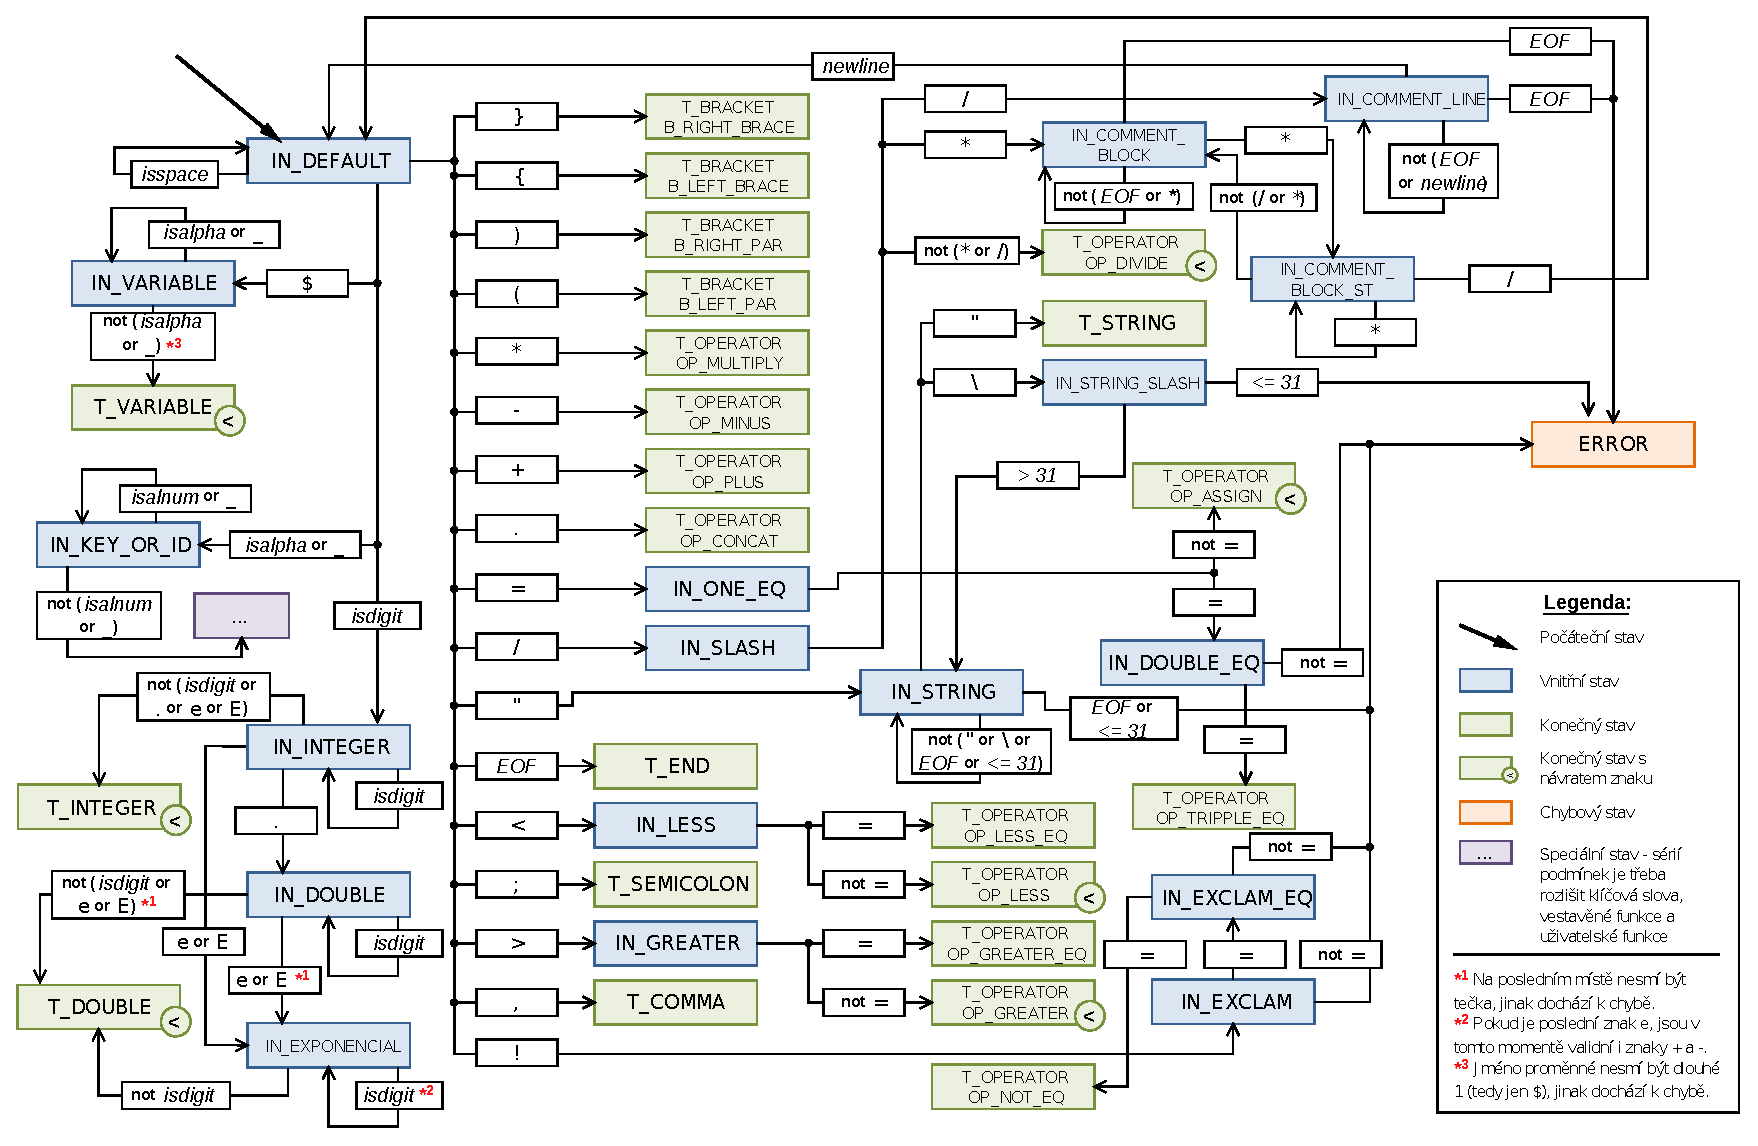
\includegraphics[angle = 90, scale = 0.75]{img/scanner.eps}
\end{center}
\end{figure}

%%%%%%%%%%%%%%%%%%%%%%%%%%%%%%%%%%%%%%%%%%%%%%%%%%%%%%%%%%%%%%%%%%%%%%%%%%%%%%%
\section{Precedenční tabulka} \label{prec_tabulka}
%%%%%%%%%%%%%%%%%%%%%%%%%%%%%%%%%%%%%%%%%%%%%%%%%%%%%%%%%%%%%%%%%%%%%%%%%%%%%%%
\begin{small}
  \newcolumntype{Y}{>{\centering\arraybackslash}X}
  \renewcommand{\arraystretch}{1.7}
  \begin{tabularx}{\textwidth}{|Y|*{16}{Y}|}
  \hline
        & $u-$ & $*$ & $/$ & $+$ & $-$ & $.$ & $<$ & $>$ & $<=$ & $>=$ & \jEQ & \nEQ & $id$ & \$  & (   & )    \\
  \hline
  $u-$    & \ME  & \VE & \VE & \VE & \VE & \VE & \VE & \VE & \VE  & \VE  & \VE  & \VE  & \ME  & \VE & \ME & \VE  \\
  $*$     & \ME  & \VE & \VE & \VE & \VE & \VE & \VE & \VE & \VE  & \VE  & \VE  & \VE  & \ME  & \VE & \ME & \VE  \\
  $/$     & \ME  & \VE & \VE & \VE & \VE & \VE & \VE & \VE & \VE  & \VE  & \VE  & \VE  & \ME  & \VE & \ME & \VE  \\
  $+$     & \ME  & \ME & \ME & \VE & \VE & \VE & \VE & \VE & \VE  & \VE  & \VE  & \VE  & \ME  & \VE & \ME & \VE  \\
  $-$     & \ME  & \ME & \ME & \VE & \VE & \VE & \VE & \VE & \VE  & \VE  & \VE  & \VE  & \ME  & \VE & \ME & \VE  \\
  $.$     & \ME  & \ME & \ME & \VE & \VE & \VE & \VE & \VE & \VE  & \VE  & \VE  & \VE  & \ME  & \VE & \ME & \VE  \\
  $<$     & \ME  & \ME & \ME & \ME & \ME & \ME & \VE & \VE & \VE  & \VE  & \VE  & \VE  & \ME  & \VE & \ME & \VE  \\
  $>$     & \ME  & \ME & \ME & \ME & \ME & \ME & \VE & \VE & \VE  & \VE  & \VE  & \VE  & \ME  & \VE & \ME & \VE  \\
  $<=$    & \ME  & \ME & \ME & \ME & \ME & \ME & \VE & \VE & \VE  & \VE  & \VE  & \VE  & \ME  & \VE & \ME & \VE  \\
  $>=$    & \ME  & \ME & \ME & \ME & \ME & \ME & \VE & \VE & \VE  & \VE  & \VE  & \VE  & \ME  & \VE & \ME & \VE  \\
  \jEQ    & \ME  & \ME & \ME & \ME & \ME & \ME & \ME & \ME & \ME  & \ME  & \VE  & \VE  & \ME  & \VE & \ME & \VE  \\
  \nEQ    & \ME  & \ME & \ME & \ME & \ME & \ME & \ME & \ME & \ME  & \ME  & \VE  & \VE  & \ME  & \VE & \ME & \VE  \\
  $id$    & \VE  & \VE & \VE & \VE & \VE & \VE & \VE & \VE & \VE  & \VE  & \VE  & \VE  & \PR  & \VE & \PR & \VE  \\
  $\$$    & \ME  & \ME & \ME & \ME & \ME & \ME & \ME & \ME & \ME  & \ME  & \ME  & \ME  & \ME  & \PR & \ME & \PR  \\
  $($     & \ME  & \ME & \ME & \ME & \ME & \ME & \ME & \ME & \ME  & \ME  & \ME  & \ME  & \ME  & \ME & \ME & \RO  \\
  $)$     & \VE  & \VE & \VE & \VE & \VE & \VE & \VE & \VE & \VE  & \VE  & \VE  & \VE  & \PR  & \VE & \PR & \VE  \\
  \hline
  \end{tabularx}
\end{small}

\begin{center}
  \begin{tabularx}{0.85\textwidth}{XXl}
  $E \rightarrow id$ & $E \rightarrow (E)$ & $E \rightarrow -E$ \\
  $E \rightarrow E*E$ & $E \rightarrow E/E$ & $E \rightarrow E+E$ \\
  $E \rightarrow E-E$ & $E \rightarrow E.E$ & $E \rightarrow E<E$ \\
  $E \rightarrow E>E$ & $E \rightarrow E<=E$ & $E \rightarrow E>=E$ \\
  $E \rightarrow E===E$ & $E \rightarrow E!==E$ & \\
  \end{tabularx}
\end{center}

%%%%%%%%%%%%%%%%%%%%%%%%%%%%%%%%%%%%%%%%%%%%%%%%%%%%%%%%%%%%%%%%%%%%%%%%%%%%%%%
\section{LL gramatika} \label{llgramatika}
%%%%%%%%%%%%%%%%%%%%%%%%%%%%%%%%%%%%%%%%%%%%%%%%%%%%%%%%%%%%%%%%%%%%%%%%%%%%%%%
\begin{center}
\begin{tabularx}{0.75\textwidth}{|llX|}
  \hline
  \rowcolor{gray!10}
  \exitem{program}     & \sipka & \textbf{\textless?php} \exitem{st-list} \\
  \hline
  \exitem{st-list}     & \sipka & \exitem{stat} \exitem{st-list} \\
  \rowcolor{gray!10}
  \exitem{st-list}     & \sipka & \slozav{\exitem{st-list}} \\
  \exitem{st-list}     & \sipka & \emph{EOF} \\
  \rowcolor{gray!10}
  \exitem{st-list}     & \sipka & \textepsilon \\
  \hline
  \exitem{stat}        & \sipka & \emph{VAR} \textbf{=} \exitem{expr}\textbf{;} \\
  \rowcolor{gray!10}
  \exitem{stat}        & \sipka & \textbf{return} \exitem{expr}\textbf{;} \\
  \exitem{stat}        & \sipka & \textbf{while} \kulzav{\exitem{expr}} \slozav{\exitem{st-list}} \\
  \rowcolor{gray!10}
  \exitem{stat}        & \sipka & \textbf{if} \kulzav{\exitem{expr}} \slozav{\exitem{st-list}} \exitem{elif-list} \\
  \exitem{stat}        & \sipka & \textbf{function} \emph{ID} \kulzav{\exitem{args}} \slozav{\exitem{st-list}} \\
  \hline
  \rowcolor{gray!10}
  \exitem{elif-list}   & \sipka & \textbf{elseif} \kulzav{\exitem{expr}} \slozav{\exitem{st-list}} \exitem{elif-list} \\
  \exitem{elif-list}   & \sipka & \textbf{else} \slozav{\exitem{st-list}} \\
  \rowcolor{gray!10}
  \exitem{elif-list}   & \sipka & \textepsilon\\
  \hline
  \exitem{args}        & \sipka & \exitem{item} \exitem{item-list} \\
  \rowcolor{gray!10}
  \exitem{args}        & \sipka & \textepsilon\\
  \hline
  \exitem{item-list}   & \sipka & \textbf{,} \exitem{item} \exitem{item-list} \\
  \rowcolor{gray!10}
  \exitem{item-list}   & \sipka & \textepsilon\\
  \hline
  \exitem{expr}        & \sipka & \emph{ID} \kulzav{\exitem{call-args}} \\
  \hline
  \rowcolor{gray!10}
  \exitem{call-args}   & \sipka & \exitem{expr} \exitem{expr-list} \\
  \exitem{call-args}   & \sipka & \textepsilon \\
  \hline
  \rowcolor{gray!10}
  \exitem{expr-list}   & \sipka & \textbf{,} \exitem{expr} \exitem{expr-list}\\
  \exitem{expr-list}   & \sipka & \textepsilon \\
  \hline
\end{tabularx}

\vspace{6pt}
Zbytek pravidel pro výrazy je pokryt v precedenční tabulce, kde výraz \emph{E}
označuje \exitem{expr} (viz~příloha \ref{prec_tabulka})
\end{center}


%%%%%%%%%%%%%%%%%%%%%%%%%%%%%%%%%%%%%%%%%%%%%%%%%%%%%%%%%%%%%%%%%%%%%%%%%%%%%%%
\section{Metriky kódu} \label{metriky}
%%%%%%%%%%%%%%%%%%%%%%%%%%%%%%%%%%%%%%%%%%%%%%%%%%%%%%%%%%%%%%%%%%%%%%%%%%%%%%%
\paragraph{Počet souborů:} 19 souborů + Makefile + dokumentace
\paragraph{Počet řádků zdrojového textu:} 6437 řádků
\paragraph{Velikost statických dat:} 161,2kB
\paragraph{Velikost spustitelného souboru:} 70,0kB (systém Linux, 64 bitová
architektura, při překla\-du bez ladicích informací, s optimalizací O3)

%%%%%%%%%%%%%%%%%%%%%%%%%%%%%%%%%%%%%%%%%%%%%%%%%%%%%%%%%%%%%%%%%%%%%%%%%%%%%%
\newpage
% seznam citované literatury: každá položka je definována příkazem
% \bibitem{xyz}, kde xyz je identifikátor citace (v textu použij: \cite{xyz})
 \begin{thebibliography}{1}

% % jedna citace:
 \bibitem{coding_style}
% Bartsch, H.~J.: 
 \emph{Linux kernel coding style}. [online] [cca 2002] [cit. 2013-12-15].
 Dostupné na:
  \texttt{\textless https://www.kernel.org/doc/Documentation/CodingStyle\textgreater}

 \bibitem{kmp_alg}
 \textsc{Lang, H.W.} \emph{Knuth-Morris-Pratt algorithm.} [online]. 
 18. srpna 2013 [cit. 2013-12-15]. Dostupné na: \\
 \texttt{\textless http://www.inf.fh-flensburg.de/lang/algorithmen/pattern/kmpen.htm\textgreater}



 \end{thebibliography}
%%%%%%%%%%%%%%%%%%%%%%%%%%%%%%%%%%%%%%%%%%%%%%%%%%%%%%%%%%%%%%%%%%%%%%%%%%%%%%

\end{document}
